\documentclass[a4paper]{article}
\usepackage[a4paper,margin=0mm]{geometry}
\usepackage{fontspec}
\usepackage{unicode-math}
\usepackage{tikz}
\usepackage[table]{xcolor}
\usepackage[absolute]{textpos}
\usepackage{enumitem}
\usepackage{array}
\usepackage{multirow}

\setmainfont{Libertinus Serif}
\setsansfont{Libertinus Sans}
\setmathfont{Libertinus Math}
\newfontfamily\trackedsans{Libertinus Sans}[LetterSpace=8.0]

\definecolor{accent}{HTML}{602785}
\definecolor{badge}{HTML}{B8A0C8}
\definecolor{ink}{HTML}{2A2E30}

\setlength{\TPHorizModule}{1mm}
\setlength{\TPVertModule}{1mm}
\setlength{\parindent}{0pt}
\pagestyle{empty}

\newcommand{\LCOL}{16mm}
\newcommand{\RCOL}{111mm}
\newcommand{\COLW}{83mm}
\newcommand{\FULLW}{178mm}

\newcommand{\topicheader}[2]{%
\begin{textblock*}{194mm}(16mm,10mm)
\begin{tikzpicture}
\node[fill=accent,text=white,font=\sffamily\bfseries\fontsize{13}{13}\selectfont,
      minimum width=9mm,minimum height=9mm,inner sep=0pt] at (4.5mm,-4.5mm) {#1};
\node[font=\sffamily\bfseries\fontsize{15}{16}\selectfont,text=ink,anchor=west] at (12mm,-4.5mm) {#2};
\end{tikzpicture}
\end{textblock*}
\begin{textblock*}{194mm}(16mm,22.5mm)

\begin{tikzpicture}
\fill[accent] (0,0) rectangle (194mm,0.5mm);
\end{tikzpicture}
\end{textblock*}
}

\newcommand{\pagefooter}[1]{%
\begin{textblock*}{194mm}(8mm,286.41mm)
  
\begin{tikzpicture}
    \fill[accent] (0,0) rectangle (194mm,0.6mm);
  \end{tikzpicture}
\end{textblock*}
\begin{textblock*}{63.59mm}(8mm,288.27mm)
  {\sffamily\bfseries\color{accent}\fontsize{13}{16}\selectfont SAT 1200+}
\end{textblock*}
\begin{textblock*}{10mm}(188mm,288.27mm)
  \centering{\sffamily\color{accent}\fontsize{14}{16}\selectfont #1}
\end{textblock*}
}

\newcommand{\colrule}[2]{%
\begin{textblock*}{1mm}(105mm,#1mm)
\begin{tikzpicture}
\draw[black!65,line width=0.5pt] (0,0) -- (0,#2mm);
\end{tikzpicture}
\end{textblock*}
}

\newcommand{\setkicker}[2]{%
{\sffamily\bfseries\fontsize{12}{14}\selectfont #1.}\ {\itshape\fontsize{11}{14}\selectfont\color{black!75} #2}\par\vspace{2mm}%
}

\setlength{\fboxsep}{1.4pt}
\setlength{\fboxrule}{0.5pt}
\newcommand{\pnum}[1]{\fcolorbox{ink}{white}{\sffamily\bfseries\fontsize{8}{8}\selectfont #1}~}

\newcommand{\qrbox}[1]{%
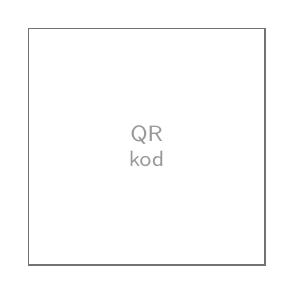
\begin{tikzpicture}
\draw[black!55,line width=0.6pt] (0,0) rectangle (30mm,30mm);
\node[black!40,font=\sffamily\fontsize{8}{9}\selectfont,align=center] at (15mm,15mm) {QR\\kod};
\end{tikzpicture}\\[1.5mm]
{\sffamily\fontsize{9}{11}\selectfont\color{black!70} #1}%
}

\arrayrulecolor{accent}
\setlength{\arrayrulewidth}{0.7pt}
\renewcommand{\arraystretch}{1.3}
\newcommand{\anstitle}[1]{{\sffamily\bfseries\color{accent}\fontsize{11}{13}\selectfont #1}\\[1.3mm]}

% ---- Answer-line for a reasoning/explanation item ----
\newcommand{\ans}[1]{{\small\color{black!75} Javob: \makebox[#1]{\dotfill}}}

\begin{document}

% ================= PAGE 1: Set 1 — Basic Frequency Table (full width) =================
\topicheader{16}{Ma'lumotlarni Taqdim Etish}
\pagefooter{84}
\mbox{}%

\begin{textblock*}{\FULLW}(16mm,30mm)
{\fontsize{11}{14}\selectfont
\setkicker{1-to'plam}{Chastota jadvalini o'qish.}

\noindent 50 nafar o'quvchidan ``Eng sevimli fan qaysi?'' deb so'ralgan:

\vspace{2mm}
\begin{center}
\begin{tabular}{|l|c|}
\hline
\rowcolor{badge!45}\textbf{Fan} & \textbf{O'quvchilar soni}\\\hline
Matematika & 18\\\hline
Fizika & 9\\\hline
Biologiya & 13\\\hline
Tarix & 10\\\hline
\rowcolor{badge!30}\textbf{Jami} & \textbf{50}\\\hline
\end{tabular}
\end{center}
\vspace{3mm}

\noindent\pnum{1} Nechta o'quvchi fizikani tanladi? \ans{35mm}\\[10mm]
\noindent\pnum{2} Matematikani tanlagan o'quvchilar jamining necha foizini tashkil qiladi? \ans{35mm}\\[10mm]
\noindent\pnum{3} Tarixni tanlagan o'quvchilar soni biologiyani tanlaganlardan nechtaga kam? \ans{35mm}\\[10mm]
\noindent\pnum{4} Fizika va tarixni tanlagan o'quvchilar birgalikda nechta? \ans{35mm}\\[10mm]
\noindent\pnum{5} Agar so'rovga yana 10 nafar o'quvchi qo'shilsa va ularning barchasi fizikani tanlasa, yangi jami nechta bo'ladi va fizikaning yangi foizi nechaga teng bo'ladi?\\
\hspace*{7mm}\ans{70mm}
}
\end{textblock*}

\clearpage

% ================= PAGE 2: Set 2 — Two-way table, row share =================
\topicheader{16}{Ma'lumotlarni Taqdim Etish}
\pagefooter{85}
\mbox{}%

\begin{textblock*}{\FULLW}(16mm,30mm)
{\fontsize{11}{14}\selectfont
\setkicker{2-to'plam}{Ikki tomonlama jadval: qator bo'yicha ulush.}

\noindent 90 nafar o'quvchidan jinsi va yoqtirgan sport turi so'ralgan:

\vspace{2mm}
\begin{center}
\begin{tabular}{|l|c|c|c|}
\hline
\rowcolor{badge!45} & \textbf{Basketbol} & \textbf{Voleybol} & \textbf{Qator jami}\\\hline
\textbf{Qizlar} & 14 & 26 & \textbf{40}\\\hline
\textbf{Yigitlar} & 33 & 17 & \textbf{50}\\\hline
\rowcolor{badge!30}\textbf{Ustun jami} & \textbf{47} & \textbf{43} & \textbf{90}\\\hline
\end{tabular}
\end{center}
\vspace{3mm}

\noindent\pnum{1} Qizlarning necha foizi voleybolni tanladi? \ans{35mm}\\[10mm]
\noindent\pnum{2} Yigitlarning necha foizi basketbolni tanladi? \ans{35mm}\\[10mm]
\noindent\pnum{3} Qizlar qator jamisining voleybolni tanlagan yigitlar soniga nisbatini eng sodda ko'rinishda yozing. \ans{35mm}\\[10mm]
\noindent\pnum{4} Yigitlarning necha foizi voleybolni tanladi? \ans{35mm}\\[10mm]
\noindent\pnum{5} Qizlar qatorida basketbol ulushi ($35\%$) bilan voleybol ulushi ($65\%$) yig'indisi nechaga teng bo'lishi SHART va nega?\\
\hspace*{7mm}\ans{70mm}
}
\end{textblock*}

\clearpage

% ================= PAGE 3: Set 3 — Same table, column share =================
\topicheader{16}{Ma'lumotlarni Taqdim Etish}
\pagefooter{86}
\mbox{}%

\begin{textblock*}{\FULLW}(16mm,30mm)
{\fontsize{11}{14}\selectfont
\setkicker{3-to'plam}{Ikki tomonlama jadval: ustun bo'yicha ulush (xuddi 2-to'plamdagi jadval).}

\vspace{2mm}
\begin{center}
\begin{tabular}{|l|c|c|c|}
\hline
\rowcolor{badge!45} & \textbf{Basketbol} & \textbf{Voleybol} & \textbf{Qator jami}\\\hline
\textbf{Qizlar} & 14 & 26 & \textbf{40}\\\hline
\textbf{Yigitlar} & 33 & 17 & \textbf{50}\\\hline
\rowcolor{badge!30}\textbf{Ustun jami} & \textbf{47} & \textbf{43} & \textbf{90}\\\hline
\end{tabular}
\end{center}
\vspace{3mm}

\noindent\pnum{1} Basketbolni tanlagan o'quvchilar ichida necha foizi qiz? \ans{35mm}\\[10mm]
\noindent\pnum{2} Voleybolni tanlagan o'quvchilar ichida necha foizi yigit? \ans{35mm}\\[10mm]
\noindent\pnum{3} 2-to'plam 1-savolning javobi ($65\%$) bilan shu yerdagi 2-savolning javobi nega bir xil emas -- ikkisi aslida bitta son emas, deb tushuntiring.\\
\hspace*{7mm}\ans{70mm}\\[4mm]
\noindent\pnum{4} Yigitlar soni jamining ($90$ dan) necha foizini tashkil qiladi? \ans{35mm}\\[10mm]
\noindent\pnum{5} ``Basketbolni tanlagan yigitlarning ulushi'' so'ralganda, qaysi sonni maxraj qilib olish kerak -- $33$, $47$, $50$ yoki $90$? Tanlovingizni asoslang va hisoblang.\\
\hspace*{7mm}\ans{70mm}
}
\end{textblock*}

\clearpage

% ================= PAGE 4: Set 4 — mixed two-way + percent context =================
\topicheader{16}{Ma'lumotlarni Taqdim Etish}
\pagefooter{87}
\mbox{}%

\begin{textblock*}{\FULLW}(16mm,30mm)
{\fontsize{11}{14}\selectfont
\setkicker{4-to'plam}{Aralash: ikki tomonlama jadval + foiz konteksti.}

\noindent 140 nafar mijozdan yosh guruhi va onlayn xariddan qoniqish darajasi so'ralgan:

\vspace{2mm}
\begin{center}
\begin{tabular}{|l|c|c|c|}
\hline
\rowcolor{badge!45} & \textbf{Qoniqdi} & \textbf{Qoniqmadi} & \textbf{Qator jami}\\\hline
\textbf{13--17 yosh} & 45 & 15 & \textbf{60}\\\hline
\textbf{18--25 yosh} & 52 & 28 & \textbf{80}\\\hline
\rowcolor{badge!30}\textbf{Ustun jami} & \textbf{97} & \textbf{43} & \textbf{140}\\\hline
\end{tabular}
\end{center}
\vspace{3mm}

\noindent\pnum{1} 18--25 yosh guruhidagilarning necha foizi qoniqmadi? \ans{35mm}\\[10mm]
\noindent\pnum{2} Qoniqmaganlar ichida necha foizi 13--17 yoshda? \ans{35mm}\\[10mm]
\noindent\pnum{3} Agar 13--17 yosh guruhi keyingi yili $20\%$ ga o'ssa, bu guruhning yangi jami nechta bo'ladi? \ans{35mm}\\[10mm]
\noindent\pnum{4} Ikki yosh guruhi orasida qoniqqanlar sonining farqi nechta -- va qaysi guruhdan qaysi guruhni ayirish kerak, musbat javob chiqishi uchun?\\
\hspace*{7mm}\ans{70mm}\\[4mm]
\noindent\pnum{5} Jadvaldagi barcha mijozlarning necha foizi umuman qoniqdi? \ans{35mm}
}
\end{textblock*}

\clearpage

% ================= PAGE 5: Set 5 — Scatterplot data =================
\topicheader{16}{Ma'lumotlarni Taqdim Etish}
\pagefooter{88}
\mbox{}%

\begin{textblock*}{\FULLW}(16mm,30mm)
{\fontsize{11}{14}\selectfont
\setkicker{5-to'plam}{Sochilish diagrammasi.}

\noindent 7 nafar talabaning haftalik mashq soati ($x$) va yugurgan masofasi, km ($y$):
$(2,4),\ (3,5),\ (4,7),\ (5,8),\ (5,10),\ (7,12),\ (8,13)$.

\vspace{3mm}
\noindent\pnum{1} $x$ oshgani sari $y$ qanday o'zgaradi -- bu qanday bog'lanish turi? \ans{50mm}\\[8mm]
\noindent\pnum{2} Ma'lumotlarda ikkita nuqta bir xil $x=5$ qiymatida, lekin turli $y$ ($8$ va $10$) ga ega. Bu real ma'lumotlar haqida nimani ko'rsatadi?\\
\hspace*{7mm}\ans{70mm}\\[6mm]
\noindent\pnum{3} Tendensiyaga asoslanib, haftasiga $6$ soat mashq qilgan talaba uchun taxminan necha km yugurish kutilishi mumkin? (Aniq son emas, oqilona oraliq bering.) \ans{40mm}\\[8mm]
\noindent\pnum{4} ``Ko'proq mashq qilish ko'proq yugurishga SABAB BO'LADI'' degan xulosa shu ma'lumotlardan to'g'ridan-to'g'ri kelib chiqadimi? Nega?\\
\hspace*{7mm}\ans{70mm}\\[6mm]
\noindent\pnum{5} Shu ma'lumotlarga asoslanib, haftasiga $25$ soat mashq qilgan talaba uchun bashorat qilish nega xavfli (qaysi tushuncha bilan bog'liq)?\\
\hspace*{7mm}\ans{70mm}
}
\end{textblock*}

\clearpage

% ================= PAGE 6: Set 6 — Spot the error (two columns, no table needed) =================
\topicheader{16}{Ma'lumotlarni Taqdim Etish}
\pagefooter{89}
\colrule{32}{238}
\mbox{}%

\begin{textblock*}{\COLW}(\LCOL,32mm)
{\fontsize{10.5}{13.5}\selectfont
\setkicker{6-to'plam}{Xatoni toping -- qaysi tushunchaga aloqador ekanini ayting, to'g'ri javobni bering.}

\noindent\pnum{1} 2--3-to'plam jadvalidan foydalaning. Savol: ``Voleybolni tanlagan o'quvchilar ichida necha foizi qiz?'' \textit{Noto'g'ri yechim:} ``$\frac{26}{40}=65\%$, demak javob $65\%$.''\\[1mm]
\hspace*{7mm}Xato va to'g'ri javob: \makebox[40mm]{\dotfill}\\[12mm]

\noindent\pnum{2} Xuddi shu jadval. Savol: ``Qizlarning necha foizi basketbolni tanladi?'' \textit{Noto'g'ri yechim:} ``$\frac{14}{90}\approx15.6\%$.''\\[1mm]
\hspace*{7mm}Xato va to'g'ri javob: \makebox[40mm]{\dotfill}
}
\end{textblock*}

\begin{textblock*}{\COLW}(\RCOL,32mm)
{\fontsize{10.5}{13.5}\selectfont
\vspace*{11.2mm}

\noindent\pnum{3} 5-to'plam ma'lumotlariga asoslanib: ``Mashq soati bilan yugurish masofasi orasida musbat bog'lanish bor, demak mashq qilish YUGURISH QOBILIYATINI OSHIRISHGA SABAB BO'LADI.''\\[1mm]
\hspace*{7mm}Xato va to'g'ri javob: \makebox[40mm]{\dotfill}\\[12mm]

\noindent\pnum{4} 4-to'plam jadvalidan foydalaning. Savol: ``Qoniqmaganlar ichida necha foizi $18$--$25$ yoshda?'' \textit{Noto'g'ri yechim:} ``$\frac{28}{80}=35\%$.''\\[1mm]
\hspace*{7mm}Xato va to'g'ri javob: \makebox[40mm]{\dotfill}
}
\end{textblock*}

\clearpage

% ================= PAGE 7: Set 7 — Bonus 3x3 table =================
\topicheader{16}{Ma'lumotlarni Taqdim Etish}
\pagefooter{90}
\mbox{}%

\begin{textblock*}{\FULLW}(16mm,30mm)
{\fontsize{11}{14}\selectfont
\setkicker{7-to'plam}{Bonus / qiyin -- $3\times3$ jadval.}

\noindent 120 nafar o'quvchidan til o'rganish usuli va erishgan natija darajasi so'ralgan:

\vspace{2mm}
\begin{center}
\begin{tabular}{|l|c|c|c|c|}
\hline
\rowcolor{badge!45} & \textbf{Past} & \textbf{O'rta} & \textbf{Yuqori} & \textbf{Qator jami}\\\hline
\textbf{Kurs usuli} & 8 & 22 & 10 & \textbf{40}\\\hline
\textbf{Ilova usuli} & 12 & 18 & 10 & \textbf{40}\\\hline
\textbf{Mustaqil usul} & 15 & 15 & 10 & \textbf{40}\\\hline
\rowcolor{badge!30}\textbf{Ustun jami} & \textbf{35} & \textbf{55} & \textbf{30} & \textbf{120}\\\hline
\end{tabular}
\end{center}
\vspace{3mm}

\noindent\pnum{1} ``Yuqori'' natijaga erishganlar ichida necha foizi ``Mustaqil usul''dan foydalangan? \ans{35mm}\\[8mm]
\noindent\pnum{2} ``Kurs usuli''dan foydalanganlarning necha foizi ``Past'' natija ko'rsatdi? \ans{35mm}\\[8mm]
\noindent\pnum{3} Har bir usul uchun alohida hisoblang: shu usuldan foydalanganlar ICHIDA ``Yuqori'' natija ko'rsatganlar ulushi (foizda) nechaga teng? Uchta javobni taqqoslang -- natija sizni ajablantiradimi?\\
\hspace*{7mm}\ans{70mm}\\[6mm]
\noindent\pnum{4} Umumiy $120$ o'quvchidan necha foizi ``O'rta'' natija ko'rsatdi? \ans{35mm}\\[8mm]
\noindent\pnum{5} ``Ilova usuli'' guruhiga yana $20$ nafar o'quvchi qo'shilsa va ularning barchasi ``Yuqori'' natija ko'rsatsa, Ilova usulining yangi jami nechta bo'ladi, va ``Yuqori'' ustunining yangi jamisi nechta bo'ladi?\\
\hspace*{7mm}\ans{70mm}
}
\end{textblock*}

\clearpage

% ================= PAGE 8: Javoblar -- unified answer table + QR =================
\topicheader{16}{Ma'lumotlarni Taqdim Etish}
\pagefooter{91}
\mbox{}%

\begin{textblock*}{194mm}(16mm,22mm)
{\bfseries\itshape\color{accent}\fontsize{19}{21}\selectfont\centering Javoblar\par}
\end{textblock*}

\begin{textblock*}{194mm}(16mm,34mm)
{\fontsize{8.7}{10.8}\selectfont
\centering
\begin{tabular}{|>{\centering\arraybackslash}p{20mm}|p{154mm}|}
\hline
\rowcolor{badge!55}\textbf{To'plam} & \textbf{Javoblar}\\
\hline
\multirow{2}{20mm}{\centering 1-to'plam} & 1)\ $9$ \quad 2)\ $36\%$ \quad 3)\ $3$ taga kam \quad 4)\ $19$\\\cline{2-2}
 & 5)\ yangi jami $=60$, fizika $=19/60\approx31.7\%$\\\hline
\multirow{2}{20mm}{\centering 2-to'plam} & 1)\ $65\%$ \quad 2)\ $66\%$ \quad 3)\ $40:17$ \quad 4)\ $34\%$\\\cline{2-2}
 & 5)\ $100\%$ -- bitta qatorning barcha ulushlari jamisi har doim butun qatorni, ya'ni $100\%$ ni beradi.\\\hline
\multirow{4}{20mm}{\centering 3-to'plam} & 1)\ $\approx29.8\%$ ($14/47$) \quad 2)\ $\approx39.5\%$ ($17/43$)\\\cline{2-2}
 & 3)\ Maxrajlar har xil -- 2-to'plam 1-savolda maxraj qizlar qator jami ($40$), bu yerda maxraj voleybol ustun jami ($43$); ikkisi boshqa-boshqa savolga javob beradi.\\\cline{2-2}
 & 4)\ $\approx55.6\%$ ($50/90$)\\\cline{2-2}
 & 5)\ Maxraj $=50$ (yigitlar qator jami) -- yigitlar guruhi ICHIDAGI ulush so'ralgan. $33/50=66\%$.\\\hline
\multirow{3}{20mm}{\centering 4-to'plam} & 1)\ $35\%$ \quad 2)\ $\approx34.9\%$ ($15/43$) \quad 3)\ $72$ ($60\times1.2$)\\\cline{2-2}
 & 4)\ $7$ -- $52-45$, katta guruhdan (18--25 yosh) kichik guruhni (13--17 yosh) ayirish kerak, aks holda manfiy javob chiqadi.\\\cline{2-2}
 & 5)\ $\approx69.3\%$ ($97/140$)\\\hline
\multirow{5}{20mm}{\centering 5-to'plam} & 1)\ Musbat bog'lanish\\\cline{2-2}
 & 2)\ Real ma'lumotlar mukammal chiziqda yotmaydi -- bir xil $x$ qiymatida turli natija bo'lishi normal\\\cline{2-2}
 & 3)\ Taxminan $10$--$12$ km oralig'ida\\\cline{2-2}
 & 4)\ Yo'q -- bog'lanish (correlation) sabab-oqibatni (causation) isbotlamaydi\\\cline{2-2}
 & 5)\ Xavfli -- bu ekstrapolyatsiya, ma'lumotlar faqat $2$--$8$ soat oralig'ini qamrab oladi.\\\hline
\multirow{4}{20mm}{\centering 6-to'plam} & 1)\ Maxraj voleybol ustun jami ($43$) bo'lishi kerak edi. To'g'ri: $26/43\approx60.5\%$.\\\cline{2-2}
 & 2)\ Maxraj qizlar qator jami ($40$) bo'lishi kerak edi. To'g'ri: $14/40=35\%$.\\\cline{2-2}
 & 3)\ Bog'lanish sabab-oqibat sifatida talqin qilingan; boshqa omillar rad etilmagan.\\\cline{2-2}
 & 4)\ Maxraj qoniqmadi ustun jami ($43$) bo'lishi kerak edi. To'g'ri: $28/43\approx65.1\%$.\\\hline
\multirow{3}{20mm}{\centering 7-to'plam} & 1)\ $\approx33.3\%$ ($10/30$) \quad 2)\ $20\%$ ($8/40$)\\\cline{2-2}
 & 3)\ Kurs: $25\%$, Ilova: $25\%$, Mustaqil: $25\%$ -- uchtasi teng (qator jamilari teng bo'lgani uchun); boshqa jadvalda bu tasodifiy bo'lmasligi mumkin.\\\cline{2-2}
 & 4)\ $\approx45.8\%$ ($55/120$) \quad 5)\ Ilova yangi jami $=60$; ``Yuqori'' ustuni yangi jamisi $=50$.\\\hline
\end{tabular}
}
\end{textblock*}

\begin{textblock*}{194mm}(16mm,246mm)
\centering
{\sffamily\fontsize{9.5}{11.5}\selectfont\color{black!70} Video yechimlar va qo'shimcha testlar uchun quyidagi QR kodlarni skanerlang:}\\[4mm]
\begin{minipage}[t]{32mm}\centering\qrbox{YouTube}\end{minipage}%
\hspace{16mm}%
\begin{minipage}[t]{32mm}\centering\qrbox{Telegram}\end{minipage}
\end{textblock*}

\end{document}
